\documentclass[11pt,a4paper]{article}
\usepackage[T1]{fontenc}
\usepackage[utf8]{inputenc}
\usepackage{lmodern,amsmath,amssymb,booktabs,array,graphicx,geometry,natbib,microtype}
\usepackage{placeins}
\usepackage[hidelinks]{hyperref}
\usepackage{fancyhdr}
\geometry{margin=24mm}
\setlength{\headheight}{14pt}
\setlength{\parskip}{1pt}
\setlength{\parindent}{1.2em}
\setlength{\emergencystretch}{2em}
\graphicspath{{../figures/}}
\usepackage{caption}
\captionsetup{font=small,labelfont=bf}
\renewcommand{\topfraction}{0.9}
\renewcommand{\bottomfraction}{0.8}
\renewcommand{\textfraction}{0.08}
\renewcommand{\floatpagefraction}{0.72}
\setcounter{topnumber}{3}
\setcounter{bottomnumber}{2}
\setcounter{totalnumber}{5}

\pagestyle{fancy}\fancyhf{}
\fancyhead[L]{\small Supplementary material: halo velocity structure}
\fancyhead[R]{}
\fancyfoot[C]{\thepage}
\newcommand{\doi}[1]{\href{https://doi.org/#1}{doi:\nolinkurl{#1}}}
\newcommand{\yv}{Y_v}
\newcommand{\Mrec}{M_{\mathrm{max,rec}}}
\newcommand{\Mterm}{M_{\mathrm{term}}}
\hypersetup{pdftitle={Supplementary material: Mass-loss dependence of accretion-history correlations in dark-matter halo velocity structure},pdfauthor={Stephen Atalebe},pdfsubject={Continuous recorded-mass-loss control, population sensitivity and structural assembly-history information}}
\title{Supplementary Material\\\large Mass-loss dependence of accretion-history correlations\\in dark-matter halo velocity structure}
\author{Stephen Atalebe\\\small Independent researcher}
\date{}
\renewcommand{\thesection}{S\arabic{section}}
\renewcommand{\thesubsection}{\thesection.\arabic{subsection}}
\renewcommand{\thetable}{S\arabic{table}}
\renewcommand{\thefigure}{S\arabic{figure}}
\renewcommand{\theequation}{S\arabic{equation}}
\begin{document}
\maketitle
\section{Formation crossings and rate processing}\label{sup:definitions}
The four-epoch routine retains positive finite masses and scale factors, sorts by scale factor and retains the first mass at each duplicate scale after sorting. It forms $\overline M$ and finds the first point satisfying $\overline M\geq f\Mrec$. At the initial sample, equality is accepted with relative tolerance $10^{-10}$ and zero absolute tolerance; otherwise a crossing already exceeded at the first sample is left-censored. Later crossings use logarithmic-mass interpolation. The additional $a_{05}/a_{90}$ routine instead combines duplicate scales by maximum mass and treats an initial value at or above threshold as censored, then joins the original four controls.

In TNG, intervals are flagged for nonfinite rates, $|r|>25$ or $|\Delta\ln M|>1$. Replacement uses the median of at least two admissible finite rates within three intervals on either side. The fallback is the median over all finite rates with $|r|\leq25$, or clipping when none exist. The BolshoiP rule requires at least five finite slopes and replaces values more than eight robust scales from the median. The scale is $1.4826$ times the median absolute deviation, with standard-deviation fallback when the deviation vanishes. These are numerical definitions rather than classifications of particular excursions as physically spurious.

\section{Numerical coverage, integration steps and design ranks}\label{sup:coverage}
\subsection{Mass ranges and direct TNG counts}
\begin{table}[htbp]\centering\small
\begin{tabular}{lrrr}
\toprule
Sample & Minimum & Median & Maximum \\
\midrule
TNG I & 10.0019 & 10.7351 & 14.6281 \\
TNG II & 10.0007 & 10.9024 & 14.3535 \\
TNG III & 10.0004 & 10.7880 & 13.8975 \\
BolshoiP I & 10.1705 & 10.5040 & 13.9057 \\
BolshoiP II & 10.1705 & 10.5101 & 14.1347 \\
BolshoiP III & 10.1705 & 10.5040 & 13.8675 \\
\bottomrule
\end{tabular}

\caption{Physical terminal-mass ranges in the available baseline populations, using each family's documented numerical convention. They do not imply equivalent halo mass definitions.}\label{tab:massranges}
\end{table}
\begin{table}[htbp]\centering\small
\begin{tabular}{lrrrr}
\toprule
 & \multicolumn{2}{c}{Endpoint count} & \multicolumn{2}{c}{Minimum along history} \\
Sample & Minimum & Median & Minimum & Median \\
\midrule
TNG I & 1,134 & 6,134.5 & 20 & 39 \\
TNG II & 1,131 & 9,018.0 & 22 & 40 \\
TNG III & 1,130 & 6,930.0 & 20 & 40 \\
\bottomrule
\end{tabular}

\caption{Direct dark-matter particle counts in the TNG trees. A small historical minimum characterizes the sampled record; it is not a convergence assessment.}\label{tab:particles}
\end{table}

\subsection{Euler multipliers}
The 26-value candidate family is
\begin{align*}
\Gamma=\{&0.2,0.3,0.5,0.8,1.2,1.8,2.6,3.0,3.5,4.0,4.25,4.5,4.75,\\
&5.0,5.25,5.5,5.75,6.0,6.5,7.0,7.5,8.0,10,12,16,20\}.
\end{align*}
For the homogeneous part of the TNG update equation in Section~3.3 of the main article, nonnegative multipliers require $\gamma\Delta\ln a\leq1$, while strict per-step contraction requires $0<\gamma\Delta\ln a<2$. All 328,172 available intervals are included in the diagnostic. The fiducial parameters satisfy the nonnegative-multiplier condition for every object. At $\gamma=4.5$, one object in TNG II and four in III have a negative multiplier; no interval in the six-point sensitivity family reaches the noncontracting threshold. At $\gamma=20$, negative multipliers occur in 420, 881 and 2,198 objects and noncontracting individual steps in 38, 92 and 180. Whole-history homogeneous products remain below one in magnitude; transient amplification and discretization error remain separate considerations.
\begin{figure}[htbp]\centering
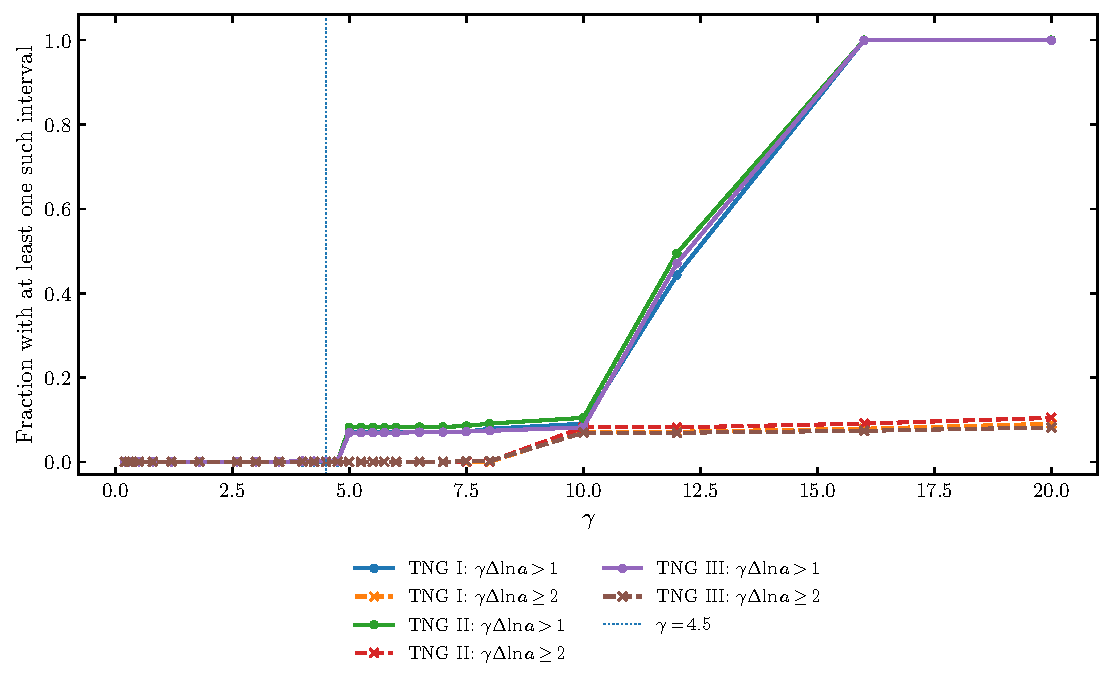
\includegraphics[width=\linewidth]{03_euler_multipliers.pdf}
\caption{Negative and noncontracting Euler-step incidence. The vertical line marks $\gamma=4.5$, the upper end of the six-point sensitivity grid. The joint-search tests use all 26 candidates.}\label{fig:euler}
\end{figure}

\subsection{Formation completeness and bracketing nodes}
All 13,517 missing BolshoiP $a_{10}$ values have first available masses above the 10 per cent threshold. This establishes finite-record left censoring. Histories containing at least one interpolated tree node number 7,675, 7,551 and 7,907 in the three available populations. Such nodes are retained. The restricted $Q_{10}\geq50$ crossing brackets contain interpolation flags in 26, 24 and 29 cases. Measured mass-equivalent brackets and time separations are available per object; no interpolated particle count is asserted.
\begin{figure}[htbp]\centering
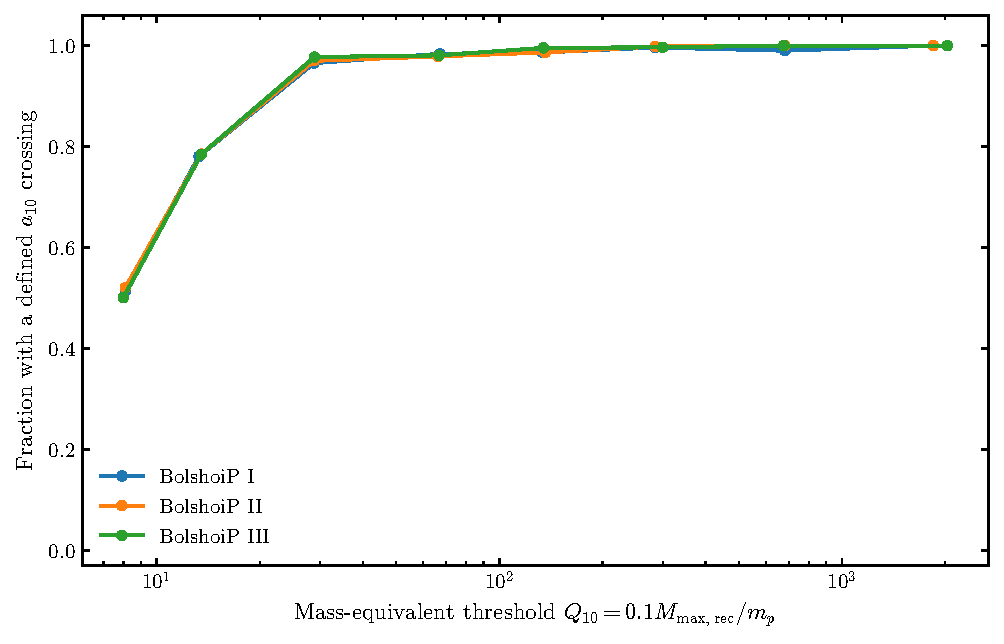
\includegraphics[width=\linewidth]{04_censoring_resolution.pdf}
\caption{Descriptive completeness in fixed bins of $Q_{10}$. Points are at within-bin medians. This relates finite-record completeness to mass scale without imposing a universal minimum-particle rule or independent-object confidence intervals.}\label{fig:censoring}
\end{figure}

\subsection{Occupied categories and numerical rank}\label{app:rank}
The four-epoch control design has an intercept, three mass powers, one current-growth term, $J-1$ indicators for $J$ occupied bins, and four epochs: $k_C=J+8$ when full rank. All nine baseline and threshold-only BolshoiP fits have $J=7$, so $k_C=15$. Table~\ref{tab:rank} reports the key populations. Their smallest physical masses cannot be read directly against bin edges defined in native $h^{-1}M_\odot$ units. At $Q_{10}\geq50$ with $L\leq2$, $\Mterm\geq3.875\times10^{10}h^{-1}M_\odot$, which empties the lowest bin and leaves six occupied categories. SVD confirms rank 14 in those three fits. All tabulated population-fit matrices have full column rank; the complete singular values and column names accompany the analysis. The rank-reducing single-observation deletion is documented separately in Section~\ref{sup:influence}.
\begin{table}[htbp]\centering\small
\begin{tabular}{llrrrr}
\toprule
Sample & Selection & Lowest-bin $n$ & Bins & Columns & Rank \\
\midrule
BolshoiP I & Baseline & 8928 & 7 & 15 & 15 \\
BolshoiP I & $Q_{10}\geq20$ & 511 & 7 & 15 & 15 \\
BolshoiP I & $Q_{10}\geq50$ & 8 & 7 & 15 & 15 \\
BolshoiP I & $Q_{10}\geq50,\ L\leq2$ & 0 & 6 & 14 & 14 \\
BolshoiP II & Baseline & 8933 & 7 & 15 & 15 \\
BolshoiP II & $Q_{10}\geq20$ & 542 & 7 & 15 & 15 \\
BolshoiP II & $Q_{10}\geq50$ & 12 & 7 & 15 & 15 \\
BolshoiP II & $Q_{10}\geq50,\ L\leq2$ & 0 & 6 & 14 & 14 \\
BolshoiP III & Baseline & 9006 & 7 & 15 & 15 \\
BolshoiP III & $Q_{10}\geq20$ & 546 & 7 & 15 & 15 \\
BolshoiP III & $Q_{10}\geq50$ & 10 & 7 & 15 & 15 \\
BolshoiP III & $Q_{10}\geq50,\ L\leq2$ & 0 & 6 & 14 & 14 \\
\bottomrule
\end{tabular}

\caption{BolshoiP control ranks and occupancy of the native $10.0$--$10.5$ logarithmic terminal-mass bin. The $Q_{10}\geq50$ threshold alone preserves the bin. Adding $L\leq2$ removes it, and the actual control rank decreases accordingly.}\label{tab:rank}
\end{table}

\section{Coefficient accounting and influence}\label{sup:influence}
Linear-loss control ranks are 17, 17 and 16 in mixed and central-only TNG and 16 in all nine BolshoiP populations. Adding the quadratic term and positive-loss indicator increases these ranks by two. Each history coordinate contributes one additional independent column. Complete ordered populations, fit summaries and numerical checks are retained with the analysis.

For native residualized variables $k_C=R_CK$ and $\ell_C=R_C\ell$, the before/after history coefficients satisfy
\begin{equation}
b_0-b_1=c\,\frac{k_C^{\mathsf T}\ell_C}{k_C^{\mathsf T}k_C}.\label{eq:ovb}
\end{equation}
This identity accounts for the coefficient change between the paired linear-loss fits on identical rows.

TNG I central-only diagnostics use the fixed 407-object predictor coordinates before and after adding $\ell$. We evaluate leverage, studentized residuals, native DFBETA and externally scaled DFBETAS using conventional OLS definitions \citep{Seabold2010}, and check them against explicit leave-one-out SVD fits. The descriptive reference $2/\sqrt{407}=0.0991$ is exceeded by 22 objects before and 17 after adjustment, including four and two of the five $L>2$ centrals. No influence threshold changes the population. One object has $|\mathrm{DFBETAS}|>1$ after adjustment; it is outside the five-object large-loss group. Every identifiable leave-one-out native history slope remains negative; after adjustment they range from $-0.03152$ to $-0.02075$.

Object 0 is the sole occupant of the highest original mass bin, $14.0$--$15.5$ in physical log mass. Its leverage is unity within numerical precision. Deleting it reduces the design rank by one in each model, so the ordinary full-rank deletion formula is undefined. Standard DFBETAS is therefore undefined for this deletion. The SVD null space is confined to nuisance directions: the history coefficient remains identifiable and unchanged to numerical precision. The other 406 deletions in each model retain rank. Explicit SVD fits evaluate all 814 individual deletions and the two joint five-object deletions.

\begin{table}[htbp]\centering\small
\begin{tabular}{rrrr}\toprule
Object ID & $\ell$ & DFBETAS before & DFBETAS after \\ \midrule
1156611 & 0.4955 & $-0.3424$ & $-0.0362$ \\
1045438 & 0.4476 & $-0.5104$ & 0.3602 \\
917708 & 0.4481 & $-0.3491$ & $-0.0064$ \\
950506 & 0.3616 & $-0.4377$ & 0.0225 \\
1072401 & 0.3049 & 0.0030 & $-0.2833$ \\
\bottomrule\end{tabular}

\caption{Individual history-coefficient influence of the five $L>2$ TNG I centrals, before and after adding $\ell$. DFBETAS uses deleted-residual variance and the full-design covariance geometry. These values are descriptive and are not summed to represent the joint group-deletion effect.}\label{tab:influence_logloss}
\end{table}

\begin{figure}[htbp]\centering
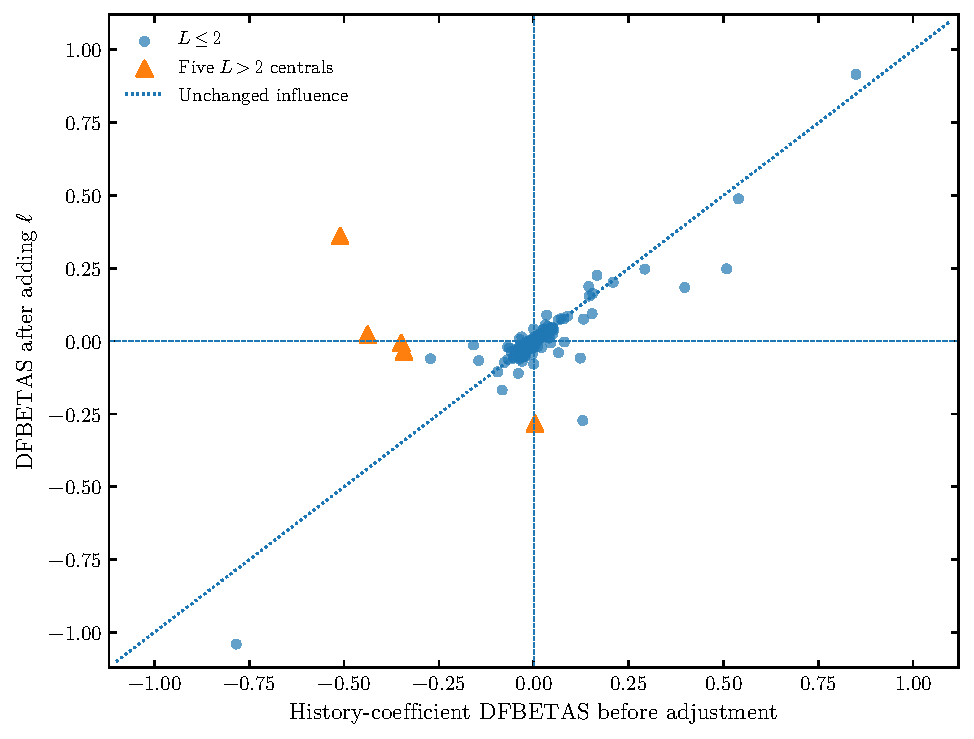
\includegraphics[width=.83\linewidth]{tng_I_influence_logL.pdf}
\caption{Change in individual history-coefficient DFBETAS for TNG I centrals. Triangles identify the five $L>2$ objects; the diagonal denotes unchanged influence. The 406 rank-preserving deletions are shown; the singleton highest-bin observation has undefined standard DFBETAS and is documented in the text. Influence is a diagnostic, not an exclusion criterion.}\label{fig:influence_logloss}
\end{figure}

\section{Mass subsets and secondary structural targets}\label{sup:secondary}
A TNG comparison splits each sample at the average BolshoiP omitted fraction, approximately $0.218$, as a mass quantile. Both subsets have negative coefficients; the lower-mass increment is larger than the full-sample increment in all three TNG samples (Table~\ref{tab:mass}). These remain descriptive diagnostics. No search-adjusted probability is assigned to these comparisons; they do not recover missing BolshoiP formation controls.
\begin{table}[htbp]\centering\small
\begin{tabular}{llrrr}\toprule
Sample & Mass subset & $n$ & $\Delta R^2_4$ & $A\pm{\rm SE}$ \\\midrule
TNG I & Lower & 92 & 0.1452 & $-0.527 \pm 0.088$ \\
TNG I & Higher & 328 & 0.0534 & $-0.287 \pm 0.038$ \\
TNG II & Lower & 192 & 0.1048 & $-0.415 \pm 0.054$ \\
TNG II & Higher & 689 & 0.0706 & $-0.357 \pm 0.028$ \\
TNG III & Lower & 479 & 0.1291 & $-0.444 \pm 0.030$ \\
TNG III & Higher & 1,720 & 0.0331 & $-0.234 \pm 0.017$ \\
\bottomrule\end{tabular}

\caption{TNG mass-subset fits with the four epochs. Errors are conventional OLS estimates. These are descriptive comparisons without a search-adjusted inference.}\label{tab:mass}
\end{table}

Secondary density and radius-related targets have separate outcomes and populations. The smallest TNG density-target fit loses the stated BIC support after formation controls, while larger TNG and BolshoiP radius-aligned comparisons retain associations. The latter use different completeness requirements. Their source tables accompany the analysis; they do not replace the $Y_v$ comparison or provide an independent profile-concentration measurement.


\section{Spatial region-deletion sensitivity}\label{supp:spatial}
Terminal coordinates are taken from \texttt{SubhaloPos} in the TNG tree files and from the terminal root rows of the BolshoiP trees. The TNG grids span $[0,75)^3\,h^{-3}\mathrm{Mpc}^3$, with cells of side $37.5$ and $25\,h^{-1}\mathrm{Mpc}$. For each BolshoiP sample, the coordinate-wise minimum and maximum of all available selected roots define a rectangular footprint before the formation-completeness cut. Its side lengths are $49.99$--$50.00\,h^{-1}\mathrm{Mpc}$, giving cells approximately $25$ and $16.7\,h^{-1}\mathrm{Mpc}$ across. These footprints are not the full $250\,h^{-1}\mathrm{Mpc}$ simulation box. No fitted result determines the boundaries.

The $2^3$ and $3^3$ grids contain no empty cells in the analysed populations. Deleting each region yields 35 fits for every population--control-design pair: 945 in total for the three mixed and three central-only TNG populations and the three formation-complete BolshoiP baseline populations, each fitted with four epochs, linear loss and flexible loss. Covariate coordinates, original mass-bin indicators and normalization remain fixed at the full-population values. For $G$ regions, we report the dispersion
\begin{equation}
 s_{\rm del}=\left[\frac{G-1}{G}\sum_{g=1}^{G}\left(b_{(-g)}-\overline b_{(-)}\right)^2\right]^{1/2}.\label{eq:sdel}
\end{equation}
Equation~\eqref{eq:sdel} is the mean-centred cluster-jackknife expression (CV3J; \citealt{MacKinnon2023}). We report it as an internal spatial scale and provide nominal reference comparisons below. Region occupancy is unequal, correlations can cross boundaries, and all regions in a family share one simulation realization. Ratios to conventional OLS standard errors compare two estimates, not two established coverage guarantees. The full range is $0.56$--$3.12$; among loss-adjusted TNG cases it is $1.22$--$2.04$. BolshoiP's 27-cell deletions remove 155--1,287 objects. No region is reweighted or preferred after inspecting the outcomes.

All 945 coefficients are negative. Twelve deletions reduce the nuisance rank when a mass-bin direction disappears; in every case the history column still adds one independent direction. The reported history slope is therefore identifiable even where the nuisance coefficients are not uniquely determined. Explicit singular-value and separate least-squares calculations agree. Table~\ref{tab:spatial} reports the flexible-loss design, while the machine-readable tables include all 54 design--grid combinations, rank changes and occupancies.
\begin{table}[htbp]\centering\footnotesize\setlength{\tabcolsep}{3pt}
\begin{tabular}{llrrrrr}
\toprule
Sample & Population & $A$ & Range: 8 cells & Range: 27 cells & 8 cells & 27 cells\\
\midrule
TNG I & mixed & $-0.1486$ & $[-0.1599, -0.1181]$ & $[-0.1762, -0.1102]$ & 1.22 & 1.80\\
TNG I & centrals & $-0.1571$ & $[-0.1745, -0.1213]$ & $[-0.1873, -0.1161]$ & 1.35 & 1.92\\
TNG II & mixed & $-0.1448$ & $[-0.1660, -0.1034]$ & $[-0.1619, -0.1218]$ & 2.04 & 1.49\\
TNG II & centrals & $-0.1588$ & $[-0.1768, -0.1168]$ & $[-0.1712, -0.1292]$ & 1.95 & 1.55\\
TNG III & mixed & $-0.0772$ & $[-0.0864, -0.0613]$ & $[-0.0847, -0.0659]$ & 1.48 & 1.52\\
TNG III & centrals & $-0.0597$ & $[-0.0695, -0.0432]$ & $[-0.0670, -0.0447]$ & 1.66 & 1.59\\
BolshoiP I & baseline & $-0.2589$ & $[-0.2697, -0.2393]$ & $[-0.2704, -0.2541]$ & 2.25 & 1.62\\
BolshoiP II & baseline & $-0.2716$ & $[-0.2775, -0.2628]$ & $[-0.2768, -0.2640]$ & 1.17 & 1.22\\
BolshoiP III & baseline & $-0.2637$ & $[-0.2832, -0.2464]$ & $[-0.2851, -0.2569]$ & 2.50 & 2.71\\
\bottomrule
\end{tabular}

\caption{Flexible-loss region-deletion sensitivity at the fiducial weighting parameter. $A$ and both deletion ranges use the full-population scaling. The two final columns are $s_{\rm del}/{\rm SE}_{\rm OLS}$ for the native history slope. Neither the ranges nor the dispersions are confidence intervals.}\label{tab:spatial}
\end{table}
\begin{figure}[htbp]\centering
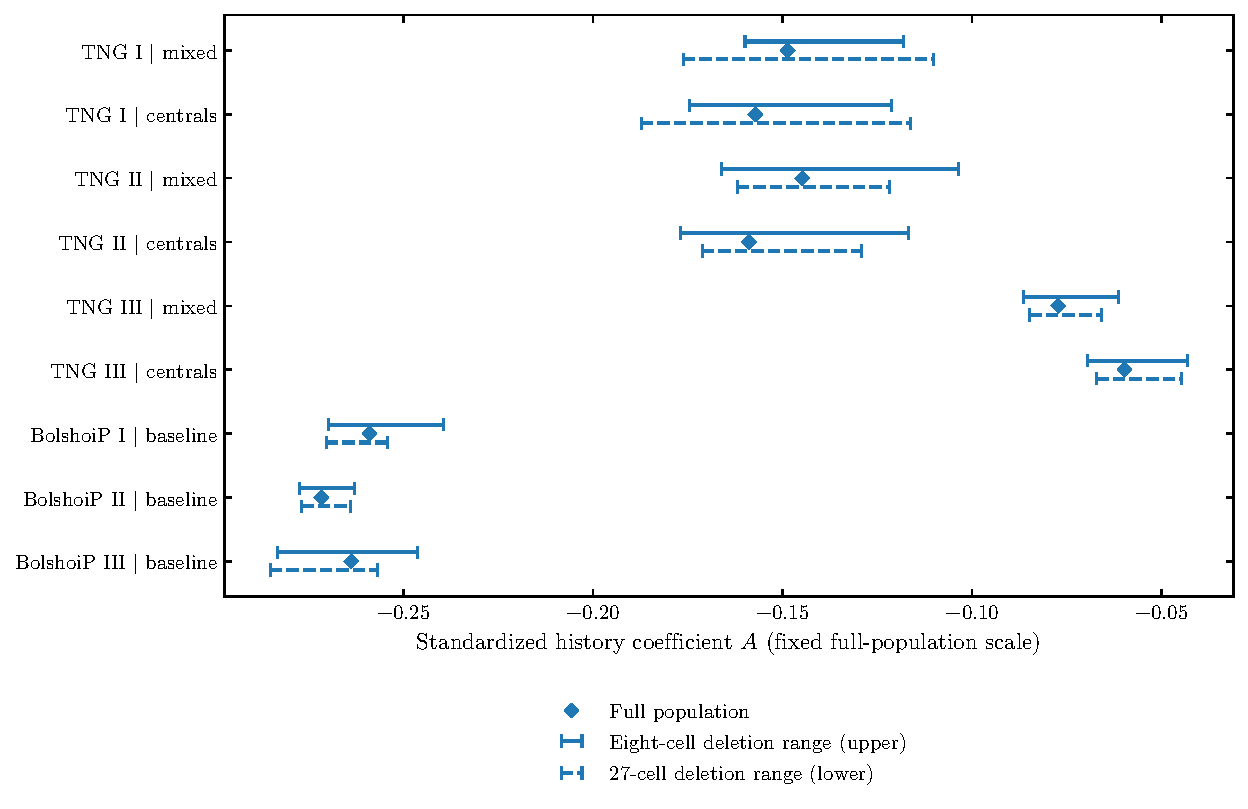
\includegraphics[width=.84\linewidth]{spatial_sensitivity.pdf}
\caption{History-coefficient ranges after deleting one region from the eight-cell or 27-cell grid, under indicator-plus-quadratic loss adjustment. Diamonds mark the full-population coefficient; horizontal segments span the extrema across deletions. These are geographic sensitivity ranges, not uncertainty intervals or additional cosmological realizations.}\label{fig:spatial}
\end{figure}

\FloatBarrier
\subsection{Nominal Student-$t$ references}\label{supp:nominal_t}
For the full-population native history slope $b$, define
\begin{align}
t_{\rm ref}&=b/s_{\rm del},\\
p_{\rm nom}&=2\Pr\!\left(T_{G-1}\geq |t_{\rm ref}|\right),\\
I_{0.95,\rm nom}&=\left[b-t_{0.975,G-1}s_{\rm del},\;b+t_{0.975,G-1}s_{\rm del}\right],
\end{align}
where $t_{0.975,G-1}$ is the 97.5th percentile of the reference Student distribution. This is a conventional working approximation with a small number of clusters; the finite-cluster reference need not be exact, and over-rejection can remain \citep{CameronMiller2015,MacKinnon2023}. The regional partition has not established the required cross-region covariance conditions. These calculations are pointwise, hold $\gamma_{\rm f}$ fixed and do not adjust for its data-informed selection, the 54 comparisons, or other model choices. The fixed-parameter spatial comparison and the global joint-search permutation comparison are separate diagnostics, not a jointly calibrated procedure.

Tables~\ref{tab:nominal8}--\ref{tab:nominal27} retain both grids and all three control designs. Here $X_{\rm flex}=[C_4,\ell,\ell^2,\mathbf1\{\ell>0\}]$. All nominal 95 per cent intervals exclude zero, but the weakest TNG loss-adjusted references are close to $0.05$. Mixed TNG I with linear loss on 27 cells has $|t_{\rm ref}|=2.1008$, $p_{\rm nom}=0.04550$ and interval $[-0.046732,-0.000509]$. TNG III centrals with flexible loss on eight cells has $|t_{\rm ref}|=2.4103$, $p_{\rm nom}=0.04675$ and interval $[-0.033755,-0.000323]$. A reference probability is not a spatial calibration or an independent confirmation. The full-precision numerical tables retain the unrounded values.

\begin{table}[p]\centering\footnotesize\setlength{\tabcolsep}{3pt}
\begin{tabular}{lllrrrl}
\toprule
Sample & Population & Controls & $b$ & $|t_{\rm ref}|$ & $p_{\rm nom}$ & Nominal 95\% interval \\
\midrule
TNG I & mixed & $C_4$ & $-0.055595$ & $15.210$ & $1.28\times10^{-6}$ & $[-0.064238, -0.046952]$ \\
TNG I & mixed & $C_4+\ell$ & $-0.023621$ & $3.096$ & $0.0174$ & $[-0.041663, -0.005578]$ \\
TNG I & mixed & $X_{\rm flex}$ & $-0.026554$ & $3.798$ & $0.0067$ & $[-0.043085, -0.010022]$ \\
TNG I & centrals & $C_4$ & $-0.044976$ & $7.365$ & $1.54\times10^{-4}$ & $[-0.059415, -0.030536]$ \\
TNG I & centrals & $C_4+\ell$ & $-0.026514$ & $3.443$ & $0.0108$ & $[-0.044726, -0.008303]$ \\
TNG I & centrals & $X_{\rm flex}$ & $-0.026594$ & $3.452$ & $0.0107$ & $[-0.044813, -0.008375]$ \\
TNG II & mixed & $C_4$ & $-0.066338$ & $5.862$ & $6.23\times10^{-4}$ & $[-0.093095, -0.039580]$ \\
TNG II & mixed & $C_4+\ell$ & $-0.026305$ & $3.021$ & $0.0194$ & $[-0.046893, -0.005717]$ \\
TNG II & mixed & $X_{\rm flex}$ & $-0.025755$ & $2.963$ & $0.0210$ & $[-0.046307, -0.005202]$ \\
TNG II & centrals & $C_4$ & $-0.042341$ & $5.306$ & $0.0011$ & $[-0.061211, -0.023471]$ \\
TNG II & centrals & $C_4+\ell$ & $-0.029783$ & $3.582$ & $0.0090$ & $[-0.049445, -0.010121]$ \\
TNG II & centrals & $X_{\rm flex}$ & $-0.028699$ & $3.237$ & $0.0143$ & $[-0.049666, -0.007731]$ \\
TNG III & mixed & $C_4$ & $-0.078149$ & $7.388$ & $1.51\times10^{-4}$ & $[-0.103160, -0.053138]$ \\
TNG III & mixed & $C_4+\ell$ & $-0.023925$ & $3.129$ & $0.0166$ & $[-0.042005, -0.005846]$ \\
TNG III & mixed & $X_{\rm flex}$ & $-0.021363$ & $3.660$ & $0.0081$ & $[-0.035164, -0.007563]$ \\
TNG III & centrals & $C_4$ & $-0.033721$ & $4.326$ & $0.0035$ & $[-0.052154, -0.015287]$ \\
TNG III & centrals & $C_4+\ell$ & $-0.018681$ & $2.865$ & $0.0242$ & $[-0.034100, -0.003261]$ \\
TNG III & centrals & $X_{\rm flex}$ & $-0.017039$ & $2.410$ & $0.0468$ & $[-0.033755, -0.000323]$ \\
BolshoiP I & baseline & $C_4$ & $-0.085302$ & $15.397$ & $1.18\times10^{-6}$ & $[-0.098402, -0.072201]$ \\
BolshoiP I & baseline & $C_4+\ell$ & $-0.067586$ & $11.199$ & $1.01\times10^{-5}$ & $[-0.081856, -0.053315]$ \\
BolshoiP I & baseline & $X_{\rm flex}$ & $-0.067188$ & $11.490$ & $8.50\times10^{-6}$ & $[-0.081015, -0.053361]$ \\
BolshoiP II & baseline & $C_4$ & $-0.087625$ & $37.699$ & $2.40\times10^{-9}$ & $[-0.093121, -0.082129]$ \\
BolshoiP II & baseline & $C_4+\ell$ & $-0.072411$ & $21.562$ & $1.16\times10^{-7}$ & $[-0.080352, -0.064470]$ \\
BolshoiP II & baseline & $X_{\rm flex}$ & $-0.071919$ & $22.856$ & $7.78\times10^{-8}$ & $[-0.079360, -0.064479]$ \\
BolshoiP III & baseline & $C_4$ & $-0.086984$ & $15.839$ & $9.69\times10^{-7}$ & $[-0.099971, -0.073998]$ \\
BolshoiP III & baseline & $C_4+\ell$ & $-0.069504$ & $10.709$ & $1.36\times10^{-5}$ & $[-0.084851, -0.054158]$ \\
BolshoiP III & baseline & $X_{\rm flex}$ & $-0.068177$ & $10.548$ & $1.50\times10^{-5}$ & $[-0.083462, -0.052893]$ \\
\bottomrule
\end{tabular}

\caption{Eight-cell nominal spatial references ($G-1=7$ reference degrees of freedom). The interval is for the native history slope at the fixed fiducial weighting parameter. Values assume the stated Student reference and are neither search-adjusted nor multiplicity-adjusted. Cross-region independence and small-cluster calibration are not established.}\label{tab:nominal8}
\end{table}
\begin{table}[p]\centering\footnotesize\setlength{\tabcolsep}{3pt}
\begin{tabular}{lllrrrl}
\toprule
Sample & Population & Controls & $b$ & $|t_{\rm ref}|$ & $p_{\rm nom}$ & Nominal 95\% interval \\
\midrule
TNG I & mixed & $C_4$ & $-0.055595$ & $6.720$ & $3.94\times10^{-7}$ & $[-0.072599, -0.038590]$ \\
TNG I & mixed & $C_4+\ell$ & $-0.023621$ & $2.101$ & $0.0455$ & $[-0.046732, -0.000509]$ \\
TNG I & mixed & $X_{\rm flex}$ & $-0.026554$ & $2.567$ & $0.0164$ & $[-0.047818, -0.005289]$ \\
TNG I & centrals & $C_4$ & $-0.044976$ & $4.504$ & $1.25\times10^{-4}$ & $[-0.065503, -0.024449]$ \\
TNG I & centrals & $C_4+\ell$ & $-0.026514$ & $2.464$ & $0.0207$ & $[-0.048631, -0.004398]$ \\
TNG I & centrals & $X_{\rm flex}$ & $-0.026594$ & $2.427$ & $0.0225$ & $[-0.049122, -0.004066]$ \\
TNG II & mixed & $C_4$ & $-0.066338$ & $5.576$ & $7.39\times10^{-6}$ & $[-0.090791, -0.041884]$ \\
TNG II & mixed & $C_4+\ell$ & $-0.026305$ & $4.196$ & $2.80\times10^{-4}$ & $[-0.039191, -0.013419]$ \\
TNG II & mixed & $X_{\rm flex}$ & $-0.025755$ & $4.068$ & $3.91\times10^{-4}$ & $[-0.038767, -0.012742]$ \\
TNG II & centrals & $C_4$ & $-0.042341$ & $6.553$ & $6.00\times10^{-7}$ & $[-0.055622, -0.029060]$ \\
TNG II & centrals & $C_4+\ell$ & $-0.029783$ & $4.224$ & $2.60\times10^{-4}$ & $[-0.044277, -0.015289]$ \\
TNG II & centrals & $X_{\rm flex}$ & $-0.028699$ & $4.076$ & $3.83\times10^{-4}$ & $[-0.043171, -0.014226]$ \\
TNG III & mixed & $C_4$ & $-0.078149$ & $6.170$ & $1.59\times10^{-6}$ & $[-0.104183, -0.052114]$ \\
TNG III & mixed & $C_4+\ell$ & $-0.023925$ & $3.838$ & $7.13\times10^{-4}$ & $[-0.036740, -0.011111]$ \\
TNG III & mixed & $X_{\rm flex}$ & $-0.021363$ & $3.575$ & $0.0014$ & $[-0.033648, -0.009079]$ \\
TNG III & centrals & $C_4$ & $-0.033721$ & $4.494$ & $1.28\times10^{-4}$ & $[-0.049145, -0.018297]$ \\
TNG III & centrals & $C_4+\ell$ & $-0.018681$ & $2.706$ & $0.0119$ & $[-0.032869, -0.004493]$ \\
TNG III & centrals & $X_{\rm flex}$ & $-0.017039$ & $2.516$ & $0.0184$ & $[-0.030959, -0.003118]$ \\
BolshoiP I & baseline & $C_4$ & $-0.085302$ & $17.160$ & $1.06\times10^{-15}$ & $[-0.095519, -0.075084]$ \\
BolshoiP I & baseline & $C_4+\ell$ & $-0.067586$ & $15.940$ & $6.16\times10^{-15}$ & $[-0.076301, -0.058870]$ \\
BolshoiP I & baseline & $X_{\rm flex}$ & $-0.067188$ & $15.963$ & $5.95\times10^{-15}$ & $[-0.075840, -0.058536]$ \\
BolshoiP II & baseline & $C_4$ & $-0.087625$ & $21.814$ & $3.08\times10^{-18}$ & $[-0.095882, -0.079368]$ \\
BolshoiP II & baseline & $C_4+\ell$ & $-0.072411$ & $21.469$ & $4.56\times10^{-18}$ & $[-0.079344, -0.065478]$ \\
BolshoiP II & baseline & $X_{\rm flex}$ & $-0.071919$ & $22.030$ & $2.41\times10^{-18}$ & $[-0.078629, -0.065209]$ \\
BolshoiP III & baseline & $C_4$ & $-0.086984$ & $12.952$ & $7.58\times10^{-13}$ & $[-0.100790, -0.073179]$ \\
BolshoiP III & baseline & $C_4+\ell$ & $-0.069504$ & $9.858$ & $2.85\times10^{-10}$ & $[-0.083997, -0.055011]$ \\
BolshoiP III & baseline & $X_{\rm flex}$ & $-0.068177$ & $9.745$ & $3.62\times10^{-10}$ & $[-0.082558, -0.053797]$ \\
\bottomrule
\end{tabular}

\caption{Twenty-seven-cell nominal spatial references ($G-1=26$ reference degrees of freedom). Definitions and qualifications are identical to Table~\ref{tab:nominal8}. Reporting both grids avoids selecting a more favourable partition; it does not supply a multiple-comparison correction.}\label{tab:nominal27}
\end{table}
\FloatBarrier
\subsection{Between-domain compatibility}\label{supp:cubes}
The three BolshoiP footprints are disjoint regions consistent with the labelled $50\,h^{-1}\mathrm{Mpc}$ tree domains. Their grids use the recorded coordinate extrema. For the three native slope estimates $b_j$ and their conventional OLS errors $s_{j,\rm OLS}$, define
\begin{equation}
 w_j=s_{j,\rm OLS}^{-2},\qquad
 \overline b_w=\frac{\sum_jw_jb_j}{\sum_jw_j},\qquad
 Q_{\rm het}=\sum_{j=1}^{3}w_j(b_j-\overline b_w)^2.
\end{equation}
Table~\ref{tab:cubes} gives a nominal $\chi^2_2$ reference for this compatibility statistic, conditional on independent estimates and correctly specified variances. The conventional OLS variances used here have not been spatially validated, and the three regions share one parent realization. A long-wavelength contribution can shift all slopes together while leaving their spread small. With only three estimates, non-rejection of heterogeneity is not a test of amplitude equivalence. The native slopes and their sample standard deviation provide a descriptive within-box comparison without that stronger interpretation.
\begin{table}[htbp]\centering\small\setlength{\tabcolsep}{3pt}
\begin{tabular}{lrrrrrr}
\toprule
Controls & $b_{\rm I}$ & $b_{\rm II}$ & $b_{\rm III}$ & Sample SD & $Q_{\rm het}$ & $p_{\chi^2,\rm nom}$ \\
\midrule
$C_4$ & $-0.085302$ & $-0.087625$ & $-0.086984$ & $0.001200$ & $0.575$ & $0.7500$ \\
$C_4+\ell$ & $-0.067586$ & $-0.072411$ & $-0.069504$ & $0.002429$ & $1.697$ & $0.4280$ \\
$X_{\rm flex}$ & $-0.067188$ & $-0.071919$ & $-0.068177$ & $0.002495$ & $1.770$ & $0.4127$ \\
\bottomrule
\end{tabular}

\caption{BolshoiP within-box slope compatibility. Sample SD uses the three native slopes and denominator two. $Q_{\rm het}$ uses inverse conventional-OLS-variance weights; its nominal probability assumes the $\chi^2_2$ reference. Neither that calculation nor agreement of the point estimates establishes independent cosmological replication or common amplitudes.}\label{tab:cubes}
\end{table}
\FloatBarrier

\section{Formation-completeness mass-bin reweighting}\label{supp:reweight}
For original native logarithmic mass stratum $b$, let $N_b$ be its available count and $n_b$ its formation-complete count. We assign every complete object in that stratum weight $w_i=N_b/n_b$. All seven strata have observed complete cases in each BolshoiP sample; no stratum is merged, trimmed or assigned an imputed formation epoch. The weights do not depend on the response, history coefficient or weighting-parameter fit. They range from 1 to 1.491, 1.473 and 1.496 in samples I--III, and sum to the respective available counts, 20,678, 20,466 and 20,929. The effective-count expression $(\sum w_i)^2/\sum w_i^2$ gives approximately 15,613, 15,603 and 15,790, respectively; it measures weight dispersion, not independent information.

Weighted least squares compares the same two nested models using the same complete objects and weights. The incremental explained variance is
\begin{equation}
\Delta R^2_w=\frac{{\rm RSS}_{C,w}-{\rm RSS}_{C+K,w}}{\sum_iw_i(Y_i-\overline Y_w)^2}.
\end{equation}
Table~\ref{tab:reweight} compares the three control designs with their unweighted counterparts. The native coefficients are directly comparable within each population; a separately standardized weighted coefficient is also supplied in the numerical results. No ordinary BIC or conventional uncertainty estimate is assigned to the weighted comparison.
\begin{table}[htbp]\centering\small
\begin{tabular}{llrrrr}
\toprule
Sample & Controls & $n$ & $b_w$ & $\Delta R^2$ & $\Delta R^2_w$\\
\midrule
BolshoiP I & $C_4$ & 16,126 & $-0.08508$ & 0.0432 & 0.0444\\
BolshoiP I & $+\ell$ & 16,126 & $-0.06702$ & 0.0199 & 0.0201\\
BolshoiP I & $+\ell,\ell^2,\mathbf1\{\ell>0\}$ & 16,126 & $-0.06654$ & 0.0195 & 0.0197\\
BolshoiP II & $C_4$ & 16,090 & $-0.08705$ & 0.0434 & 0.0440\\
BolshoiP II & $+\ell$ & 16,090 & $-0.07163$ & 0.0210 & 0.0209\\
BolshoiP II & $+\ell,\ell^2,\mathbf1\{\ell>0\}$ & 16,090 & $-0.07106$ & 0.0205 & 0.0203\\
BolshoiP III & $C_4$ & 16,340 & $-0.08619$ & 0.0453 & 0.0461\\
BolshoiP III & $+\ell$ & 16,340 & $-0.06890$ & 0.0202 & 0.0205\\
BolshoiP III & $+\ell,\ell^2,\mathbf1\{\ell>0\}$ & 16,340 & $-0.06745$ & 0.0192 & 0.0194\\
\bottomrule
\end{tabular}

\caption{Mass-bin reweighting of observed formation-complete BolshoiP objects, all at $\gamma_{\rm f}=1.2$. The control designs are four formation epochs ($C_4$), $C_4+\ell$, and $C_4+\ell+\ell^2+\mathbf1\{\ell>0\}$. $b_w$ is the weighted native-unit history slope. No missing formation value is reconstructed.}\label{tab:reweight}
\end{table}

The complete-minus-available mean native log-mass offsets are 0.0894, 0.0860 and 0.0915 dex before weighting and 0.0212, 0.0208 and 0.0223 dex afterward. Matching coarse mass-bin counts therefore improves mass balance without eliminating differences within those bins. All 13,517 omitted $a_{10}$ values are left-censored: their crossings precede the first available point. Reweighting characterizes the sensitivity to the observed mass-stratum distribution; it does not establish missing-at-random selection, determine the missing epochs, or identify either the sign or magnitude of bias in the unavailable full-population four-epoch regression. A quantitative bound on that regression would require additional restrictions on the missing histories and model.

{\small
\begin{thebibliography}{9}
\bibitem[Cameron \& Miller(2015)]{CameronMiller2015}
Cameron A. C., Miller D. L., 2015, Journal of Human Resources, 50, 317--372. A practitioner's guide to cluster-robust inference. \doi{10.3368/jhr.50.2.317}

\bibitem[MacKinnon et al.(2023)]{MacKinnon2023}
MacKinnon J. G., Nielsen M. {\O}., Webb M. D., 2023, Journal of Applied Econometrics, 38, 671--694. Fast and reliable jackknife and bootstrap methods for cluster-robust inference. \doi{10.1002/jae.2969}

\bibitem[Seabold \& Perktold(2010)]{Seabold2010}
Seabold S., Perktold J., 2010, in Proceedings of the 9th Python in Science Conference, pp. 92--96. Statsmodels: Econometric and statistical modeling with Python. \doi{10.25080/Majora-92bf1922-011}

\end{thebibliography}
}
\end{document}
